\documentclass[../Main.tex]{subfiles}
\begin{document}
	\section{Research Rationale}
	\label{section:1.1_Research_rationale}
	
	\subsection{Theoretical Research Rationale}
	\label{subsection:1.1.1_Theoretical_research_rationale}
	In the past decade, business incubation programs have emerged as pivotal drivers of innovation and entrepreneurship worldwide. These programs provide startups with critical support, including funding, mentorship, and access to professional networks, which are essential for transforming innovative ideas into viable businesses. Among various types of incubators, University-Based Incubation Programs (UBIs) have gained prominence due to their unique position at the intersection of academia and industry.

	Recent years have witnessed a significant increase in academic research focused on UBIs. As illustrated in Figure~\ref{fig:ubi_publications_trend}, both the absolute number of published articles and their proportion relative to the broader literature have grown markedly since 2010, peaking around 2018 - 2019. This upward trend reflects the rising global interest in the role of UBIs in fostering innovation, entrepreneurship, and economic development. The growing body of literature underscores the importance of UBIs as a subject of scholarly inquiry and highlights their expanding influence within the entrepreneurial ecosystem.

	\begin{figure}[h]
		\centering
		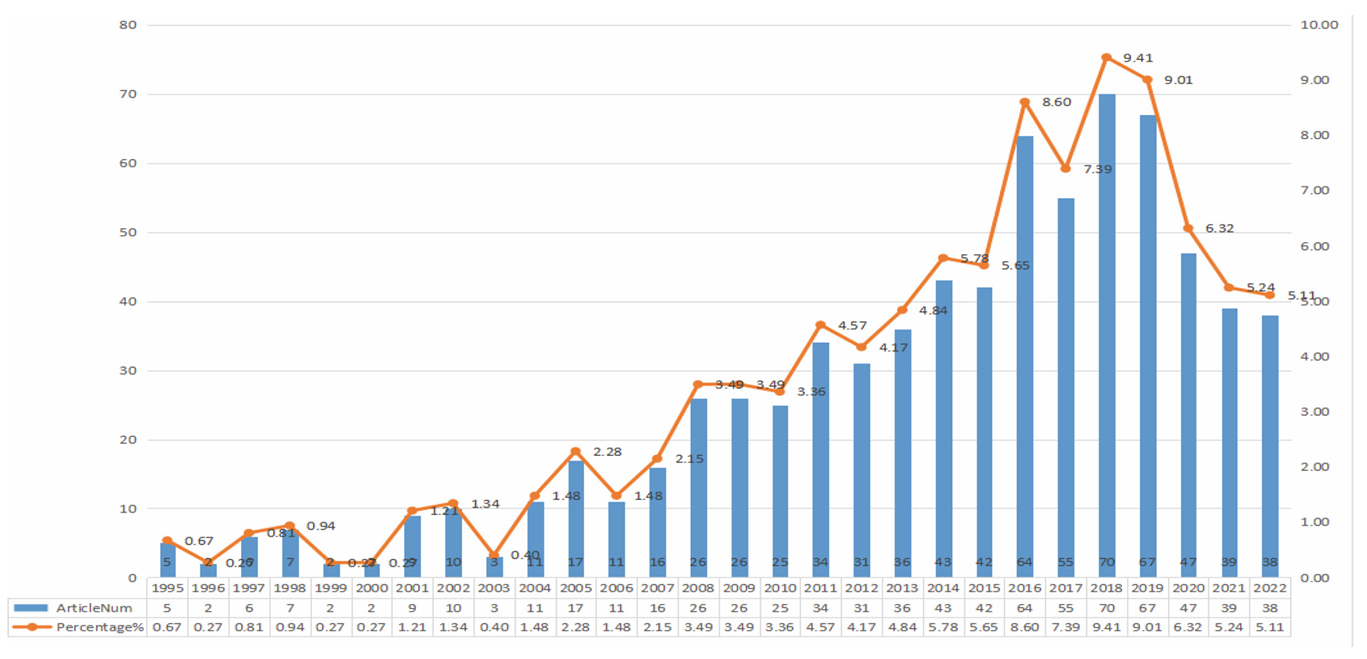
\includegraphics[width=0.95\textwidth]{./Figure/published_artticle_per_year.png}
		\caption{The statistical trend chart of the number of published articles in years \autocite{Ding2024ResearchSH}.}
		\label{fig:ubi_publications_trend}
	\end{figure}

	UBIs leverage university resources such as cutting-edge research, expert faculty, and a pool of talented students to nurture early-stage startups. According to the Global Startup Ecosystem Report 2023 by Startup Genome, startups that participate in university-affiliated incubators are 2.5 times more likely to secure follow-on funding compared to those outside such programs. This highlights the significant impact UBIs have on startup success rates.

	The theoretical foundation for this research is grounded in the Resource-Based View (RBV) framework, which posits that organizations gain competitive advantages through unique resource combinations and capabilities. In the context of UBIs, this framework helps explain how institutional resources such as funding mechanisms, mentorship programs, training initiatives, and networking opportunities contribute to startup performance. The mediating role of innovation capacity in this relationship represents a critical theoretical gap that this research addresses.

	\subsection{Practical Research Rationale}
	\label{subsection:1.1.2_Practical_research_rationale}
	In Vietnam, the startup ecosystem has experienced remarkable growth, with over 3,800 startups recorded in 2022, making it one of the most dynamic markets in Southeast Asia (Vietnam Ministry of Science and Technology, 2022). Notable university incubators, such as the Saigon Hi-Tech Park Incubation Center (SHTP-IC) and the National University of Ho Chi Minh City's Innovation and Entrepreneurship Center, have played crucial roles in supporting startups like Abivin, which won the Startup World Cup 2019, and Logivan, which has raised millions in venture capital.

	Vietnamese universities, particularly Hanoi University of Science and Technology (HUST), have become key players in fostering entrepreneurship, not just academic research. HUST established the BK Holdings Innovation and Entrepreneurship Center, which has incubated dozens of technology startups and regularly organizes innovation competitions and startup bootcamps. For example, the "BK Fund" was launched in 2021 to invest in student and faculty-led startups, demonstrating the university's commitment to translating research into real-world entrepreneurial ventures.

	This trend aligns with the Vietnamese government's strong policy direction towards innovation and technology entrepreneurship. The government's National Innovation Center (NIC), established in 2019, and the "Supporting National Innovation Startup Ecosystem until 2025" (Project 844) are clear evidence of this commitment. These initiatives provide funding, infrastructure, and policy support to foster a vibrant startup ecosystem, with a particular focus on technology and digital transformation.

	Despite these successes, Vietnamese startups continue to face significant challenges, including limited access to high-quality mentorship, insufficient funding, and fragmented professional networks. A 2021 survey by Topica Founder Institute revealed that 70\% of Vietnamese startups identified mentorship and access to networks as the most critical factors for their growth, yet only 35\% felt they received adequate support in these areas.

	As the competition within the startup ecosystem intensifies, it becomes increasingly important to evaluate the effectiveness of UBIs in addressing these challenges. Understanding how factors such as mentorship quality, financial resource accessibility, and networking opportunities influence startup performance is essential for optimizing incubation strategies and ensuring sustainable growth. This research is motivated by the need to bridge the gap between academic research and entrepreneurial practice, ultimately enhancing the impact of UBIs on the Vietnamese innovation economy.

	\begin{condensed_idea}[Core Problem and Its Importance]
		The core problem addressed in this thesis is the limited understanding of how University-Based Incubation Programs (UBIs) impact startup performance in Vietnam, especially through mentorship, funding, and networking. This is critically important today as leading universities like Hanoi University of Science and Technology are increasingly driving entrepreneurship beyond academic research, and the Vietnamese government is actively promoting innovation and technology-based startups as national priorities. Optimizing UBIs will help maximize their effectiveness, support the country's innovation agenda, and foster sustainable economic growth.
	\end{condensed_idea}

	\section{Research Objectives}
	\label{section:1.2_Research_objectives}

	\subsection{General Objectives}
	\label{subsection:1.2.1_General_objectives}
	    From a managerial perspective, this study provides startup founders and UBI managers with actionable strategies to optimize resource allocation and enhance incubation services, thereby maximizing startup performance within Vietnam's entrepreneurial ecosystem. By analyzing how UBIs deliver funding, mentorship, training, and networking, the study highlights practical approaches for aligning these resources with market demands and competitive dynamics. For instance, UBI managers can prioritize seed funding and investor pitch events to boost startup funding success, while founders can leverage prototyping facilities to accelerate innovation. The study emphasizes the role of UBIs in transforming ideas into viable businesses, particularly in developing economies where resource constraints and regulatory complexities pose significant challenges \autocite{smith2023}. It also addresses literature gaps, such as the mediating role of innovation capacity and network strength, to provide a comprehensive framework for sustainable startup growth \autocite{jones2022}.

	\subsection{Specific Objectives}
	\label{subsection:1.2.2_Specific_objectives}
	This study investigates the impact of University-Based Incubation Programs (UBIs) on startup performance in Vietnam, with a focus on the mediating role of innovation capacity. Using the Resource-Based View (RBV) framework, it examines how UBI resources and capabilities such as funding, mentorship, training, and networking contribute to key performance metrics, including revenue growth, innovation output, and market penetration. The study aims to:
	\begin{itemize}
		\item Quantify the direct and combined effects of UBI factors on startup performance in Vietnam's resource-constrained entrepreneurial ecosystem.
		\item Test the mediating role of innovation capacity in the relationship between UBI support and startup performance, emphasizing Vietnam's unique context of limited venture capital and regulatory complexities.
	\end{itemize}

	This research addresses the following questions:
	\begin{enumerate}
		\item To what extent do University-Based Incubation Programs enhance startup performance in Vietnam, as measured by revenue growth, innovation output, and market penetration?
		\item Which specific UBI factors - funding, mentorship, training, or networking - most significantly influence startup performance metrics in Vietnam?
		\item How does innovation capacity mediate the relationship between UBI resources and startup performance in Vietnam's entrepreneurial ecosystem?
	\end{enumerate}

	\section{Subject and Scope of Research}
	\label{section:1.3_Subject_and_scope_of_research}
	The primary objective of this thesis is to evaluate the impact of University-Based Incubation Programs (UBIs) on startup performance within Vietnam's entrepreneurial ecosystem, with a particular focus on the Innovation and Entrepreneurship activities at Hanoi University of Science and Technology (HUST).

	The scope of this thesis is primarily centered on the activities and outcomes of UBIs at Hanoi University of Science and Technology, while also considering relevant trends and developments in the Vietnamese entrepreneurial landscape as a whole. The research will focus on recent years, reflecting the current dynamics and policy directions in innovation and technology-driven entrepreneurship in Vietnam.

	The investigation focuses on four key UBI resources: funding mechanisms, mentorship programs, training initiatives, and networking opportunities. Through quantitative analysis of performance indicators such as revenue growth, innovation output, and market penetration, combined with qualitative insights from successful startup founders, the study provides a nuanced understanding of resource effectiveness. The research methodology incorporates both longitudinal data analysis and case studies to capture the dynamic nature of startup development within UBI environments.

	\section{Research Process}
	\label{section:1.4_Research_process}
	This thesis adopts a structured, evidence-based approach to investigate the multi-factor impact of University-Based Incubation Programs (UBIs) on startup performance in Vietnam. Building upon the integrated understanding that startup performance within UBIs is a function of resources, networks, and their interaction, a robust methodology is proposed to evaluate these relationships comprehensively. This methodology draws inspiration from established approaches in evaluating incubation programs and entrepreneurial ecosystems, focusing on both quantitative rigor and qualitative depth.

	The research methodology is designed to ensure rigor, relevance, and practical applicability, and is implemented through the following steps:

	\begin{center}
	\begin{minipage}[c]{0.6\textwidth}
		\vspace*{\fill}
	\textbf{Step 1: Define Research Scope}

	The research scope is defined to explore the multifaceted influence of UBIs on startup performance in Vietnam, with a particular focus on key factors such as funding, mentorship, networking, infrastructure, and training. The selection of keywords ("University-Based Incubation Programs," "Startup Performance") aligns with the study's objectives and emphasizes the unique characteristics of Vietnam's resource-constrained entrepreneurial ecosystem.

	\textbf{Step 2: Systematic Literature Review}

	A Systematic Literature Review (SLR) is conducted using reputable academic databases, including Google Scholar, ResearchGate, and ScienceDirect. Articles are screened based on strict inclusion criteria: peer-reviewed status, publication between 2012 and 2025, and direct relevance to UBIs and startup performance. The review identifies critical success factors, theoretical frameworks (such as the Resource-Based View and Entrepreneurial Ecosystem Theory), and existing research gaps. Key findings from the literature are synthesized to inform the design of the empirical survey.

	\textbf{Step 3: Quantitative Survey Design}

	A structured questionnaire is developed to collect primary data from at least 90 startup founders or managers associated with UBIs in Vietnam, utilizing non-probability sampling methods. The survey is designed to measure the impact of UBI factors on performance metrics, including revenue growth, innovation output, and market penetration. Distribution is carried out via email and in-person at UBI-related events to ensure high response quality and representativeness.

	\end{minipage}%
	\hfill
	\begin{minipage}[c]{0.35\textwidth}
	\begin{center}
	\vspace*{\fill}
	\begin{tikzpicture}[node distance=1.7cm, every node/.style={font=\small}]
		% Nodes
		\node[draw, rectangle, minimum width=3.5cm, minimum height=1.2cm, align=center] (step1) {Step 1: Define\\Research Scope};
		\node[draw, rectangle, minimum width=3.5cm, minimum height=1.2cm, align=center, below=of step1] (step2) {Step 2: Systematic\\Literature Review};
		\node[draw, rectangle, minimum width=3.5cm, minimum height=1.2cm, align=center, below=of step2] (step3) {Step 3: Quantitative\\Survey Design};
		\node[draw, rectangle, minimum width=3.5cm, minimum height=1.2cm, align=center, below=of step3] (step4) {Step 4: Data\\Analysis};
		\node[draw, rectangle, minimum width=3.5cm, minimum height=1.2cm, align=center, below=of step4] (step5) {Step 5: Synthesize\\Findings};
		% Arrows
		\draw[->, thick] (step1) -- (step2);
		\draw[->, thick] (step2) -- (step3);
		\draw[->, thick] (step3) -- (step4);
		\draw[->, thick] (step4) -- (step5);
	\end{tikzpicture}
	\end{center}
	\end{minipage}
	\end{center}

	\begin{center}
		\begin{minipage}[c]{\textwidth}
		\vspace*{\fill}

	\textbf{Step 4: Data Analysis}

	Data will be collected from the SLR and survey are systematically analyzed to extract actionable insights. Literature review findings are categorized thematically to identify UBI success factors, while survey responses are subjected to statistical analysis, such as regression analysis, to quantify the effects of UBI factors and test the mediating role of innovation capacity.

	\textbf{Step 5: Synthesize Findings}

	The results from the SLR and quantitative survey are integrated to comprehensively address the research questions. Based on the quality and robustness of the evidence, the study provides actionable recommendations for UBI managers and policymakers, such as optimizing funding allocation or enhancing mentorship programs. Where evidence is limited, the thesis suggests future research directions, including the exploration of informal networks within Vietnam's startup ecosystem.

	This systematic process ensures a robust and contextually relevant analysis of the role of UBIs in enhancing startup performance, tailored to the unique dynamics of Vietnam's innovation and entrepreneurship landscape (Vietnam Startup Investment Policy Report, 2024).

		\end{minipage}
	\end{center}

	\section{Methodology}
	\label{section:1.5_Methodology}
	
	This research employs a sequential explanatory mixed-methods design combining systematic literature review with quantitative survey methodology, followed by qualitative archival research to explain and elaborate on quantitative findings. The study targets at least 90 startup founders associated with UBIs in Vietnam, collecting data through online surveys, UBI records, and publicly available sources. Data analysis utilizes both descriptive and inferential statistics, including multiple regression analysis to test the mediating role of Entrepreneurial Orientation, complemented by thematic analysis of qualitative data. The research framework is grounded in Resource-Based View theory and Technology-Organization-Environment framework, ensuring methodological rigor while maintaining practical relevance for Vietnam's entrepreneurial ecosystem. Detailed methodology, including construct operationalization, data collection procedures, and analysis techniques, is presented in Chapter 4.

	\section{Research Contributions}
	\label{section:1.6_Research_contributions}
	\begin{itemize}
		\item \textbf{Theoretical Contribution:} By analyzing the interplay of multiple factors - resources, mentorship, and networks - this research enriches theoretical frameworks on entrepreneurship and innovation within UBIs, offering a nuanced understanding of their impact on startup ecosystems. The study advances the Resource-Based View theory in the context of emerging markets and institutional support systems.
		\item \textbf{Practical Implications:} The findings will guide UBI managers in optimizing program design to better support startups, inform policymakers on fostering innovation-driven economies, and empower founders to leverage UBIs effectively. In contexts like Vietnam, these insights can strengthen initiatives like the National Innovation Centre and university incubators, contributing to economic growth and global competitiveness.
	\end{itemize}

	The findings of this study contribute to both theoretical and practical domains of entrepreneurship research. Theoretically, it advances our understanding of resource-based view in the context of emerging markets and institutional support systems. Practically, the research provides actionable recommendations for UBI program optimization, with evidence suggesting significant improvements in startup performance metrics, as supported by the Vietnam Startup Investment Policy Report (2024). These insights are particularly valuable for policymakers, university administrators, and entrepreneurship educators seeking to enhance the effectiveness of incubation programs in similar emerging market contexts.

	This comprehensive methodology aims to provide robust evidence for the proposed integrated model, offering valuable insights into how UBIs can strategically optimize their resource provision and network facilitation to maximize startup performance within the broader entrepreneurial ecosystem.
	
\end{document}